
\documentclass[12pt]{article}
\usepackage[margin=1in]{geometry}
\usepackage[pdftex]{graphicx}
\usepackage{multirow}
\usepackage{setspace}
\usepackage{enumitem}
\pagestyle{plain}
\setlength\parindent{0pt}

\begin{document}

% Course information
\begin{tabular*}{\textwidth}{l @{\extracolsep{\fill}} r}
  & \multirow{3}{*}{
\includegraphics[height=1.0in]{logo.jpg}} \\
  \large 116C Title & \\
  \large Spring Quarter 2018 & \\
  \large Physics 116C & \\
\end{tabular*}
\vspace{10mm}

% Professor information
\begin{tabular}{ l l }
  \multirow{6}{*}{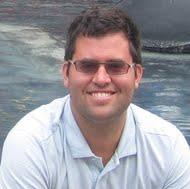
\includegraphics[height=1.25in]{mike.jpg}} & \\
  & \\
  & \large Michael Mulhearn \\
  & \large mulhearn@physics.ucdavis.edu \\
  & \large Physics 317 \\
  & \\
\end{tabular}
\vskip 0.5cm
\noindent
\textbf {Lectures:} M,W,F 12:10-1:00 PM in Rm. 140 Physics
\begin{tabbing}
\hspace*{3em}\= \hspace*{5em} \= \kill % set the tabbings
\textbf {Lab:}    \> Section 1: \>  M 2:10-5:00 PM in Rm. 152 Roessler \\
                        \> Section 2: \> W 3:10-6:00 PM in Rm. 152 Roessler \\
\end{tabbing}

\noindent
\textbf {Texts:} \emph{The Art of Electronics}, 3\textsuperscript{rd} Edition, Horowitz and Hill\\
\emph{An Introduction to Error Analysis}, 2\textsuperscript{nd} Edition, John R. Taylor\\
{\tt https://www.scipy-lectures.org/\_downloads/ScipyLectures-simple.pdf} \\
\noindent
\textbf{Office Hours:} W 2:00-3:00 PM in 152 Roessler, and also often available during most lab sessions.\\
\noindent
\textbf{Lab Instructor:} Christopher Brainerd, cbbrainerd@ucdavis.edu \\
\noindent
\textbf{Midterm Exams:} Two Midterm Exams:  \\ 
These will be in-class, due to cheating in the spring quarter.  Tentative date for first midterm in 4 May.\\

\textbf{Final Exam:} June 11, 2018 at 6:00 PM in Physics 140 \\
\textbf{Homework:}  There will be approximately five homework assignments.\\

\noindent
\textbf {Course Description:}  
Use of computing in physics experimentation.  The normal, binomial, and poisson distributions;  the propagation and statistical analysis of experimental uncertainties;  least squares fitting; Fourier transforms.\\

\noindent
\textbf {Course Objections:} 
You will gain proficiency in Arduino microprocessor programing and data analysis with Scientific Python.\\

\noindent
\textbf {Lab Safety:} 
You should complete the online course for Electrical Safety at \\
{\tt http://safetyservices.ucdavis.edu/training/electrical-safety}.\\

\noindent
\textbf {Lab Reports:} 
There will be three long lab reports for the Geiger Lab, Johnson Noise Lab, and the (floating) Muon Lifetime lab.  The remaining labs include instructions for a report, generally much shorter with fewer requirements.

\vskip 0.5cm
\noindent
\textbf {Tentative Course Outline}:

The weekly coverage might change as it depends on the progress of the class.    Most weeks we'll need to cover some additional material to prepare for the upcoming labs.



\begin{table}[h!]
\normalsize % The size of the table text can be changed depending on content. Remove if desired.
\begin{tabular}{ llll }
\hline
\textbf{Week} & \textbf{Dates} & \textbf{Lecture} & \textbf{Lab} \\
\hline
1 & 2,4,6 Apr & Microprocessors and Assembly & 1) Intro to Arduino and Scipy \\
\hline
2 & 9,11,13 Apr &  & 2) Arduino Function Generator \\
\hline
3 & 16,18,20 Apr & Statistical Distributions & 3) Arduino Digital Scope  \\
\hline
4 & 23,25,27 Apr & Uncertainties & 4) Geiger Counter \\
\hline
5 & 30 Apr 2,4 May & Fourier Transform & 4) Geiger Counter \\
\hline
6 & 7,9,11 May & Noise & 5) Fast Fourier Transform \\
\hline
7 & 14,16,18 May & Statistical Analysis  & 6) Johnson Noise \\
\hline
8 & 21,23,25 May & & 6) Johnson Noise\\
\hline
9 & (28),30 May,1 Jun & &  No Lab \\
\hline
10 &  4,6 Jun &  & 7)  Arithmetic Logic Unit\\
\hline
\end{tabular} 
\end{table}

\end{document}

